\chapter{Equilíbrios ácido--base e o método da reação predominante}\label{ch:b1:predominant-reaction}

O vinagre dissolve o calcário de uma chaleira; o suco de limão também, um
pouco mais depressa. O sangue mantém seu pH dentro de limites estreitos,
seja o que for que comamos; um refrigerante é ácido por causa do dióxido
de carbono dissolvido nele. Todos esses são equilíbrios ácido--base em
água, e o químico diante de uma solução que contém vários ácidos e bases
--- uma mistura, um tampão, um \omterm{def:b1:predominant-reaction:polyprotic}{poliácido} --- precisa de um método
confiável para encontrar seu pH e as concentrações de suas espécies.
Este capítulo constrói esse método: uma escala de forças, \omterm{def:b1:predominant-reaction:predominance}{diagramas de
predominância} e o \emph{método da \omterm{def:b1:predominant-reaction:predominant-reaction}{reação predominante}}, que reduz
qualquer mistura à única reação que importa.

\begin{recall}
O Livro 1 (ano 12) definiu os ácidos e as \omterm{def:b1:predominant-reaction:bronsted}{bases de Brønsted}, a \omterm{def:b1:predominant-reaction:acidity-constant}{constante
de acidez} $K_a$ e o $\mathrm{p}K_a$, o \omterm{def:b1:predominant-reaction:autoprotolysis}{produto iônico da água} e o pH dos
ácidos e das \omterm{def:b1:predominant-reaction:strong-acid}{bases fortes}, e traçou \omterm{def:b1:predominant-reaction:predominance}{diagramas de predominância}. O
\omterm{def:b1:extent-q-and-k:quotient}{quociente de reação}, a constante de equilíbrio e as \omterm{def:b1:extent-q-and-k:activity}{atividades} dos
solutos ($c/c^\circ$) e do solvente (1) foram definidos no
\cref{ch:b1:extent-q-and-k}; neste capítulo, $c^\circ = \qty{1}{mol/L}$
não é escrito nos quocientes.
\end{recall}

\begin{omfigure}
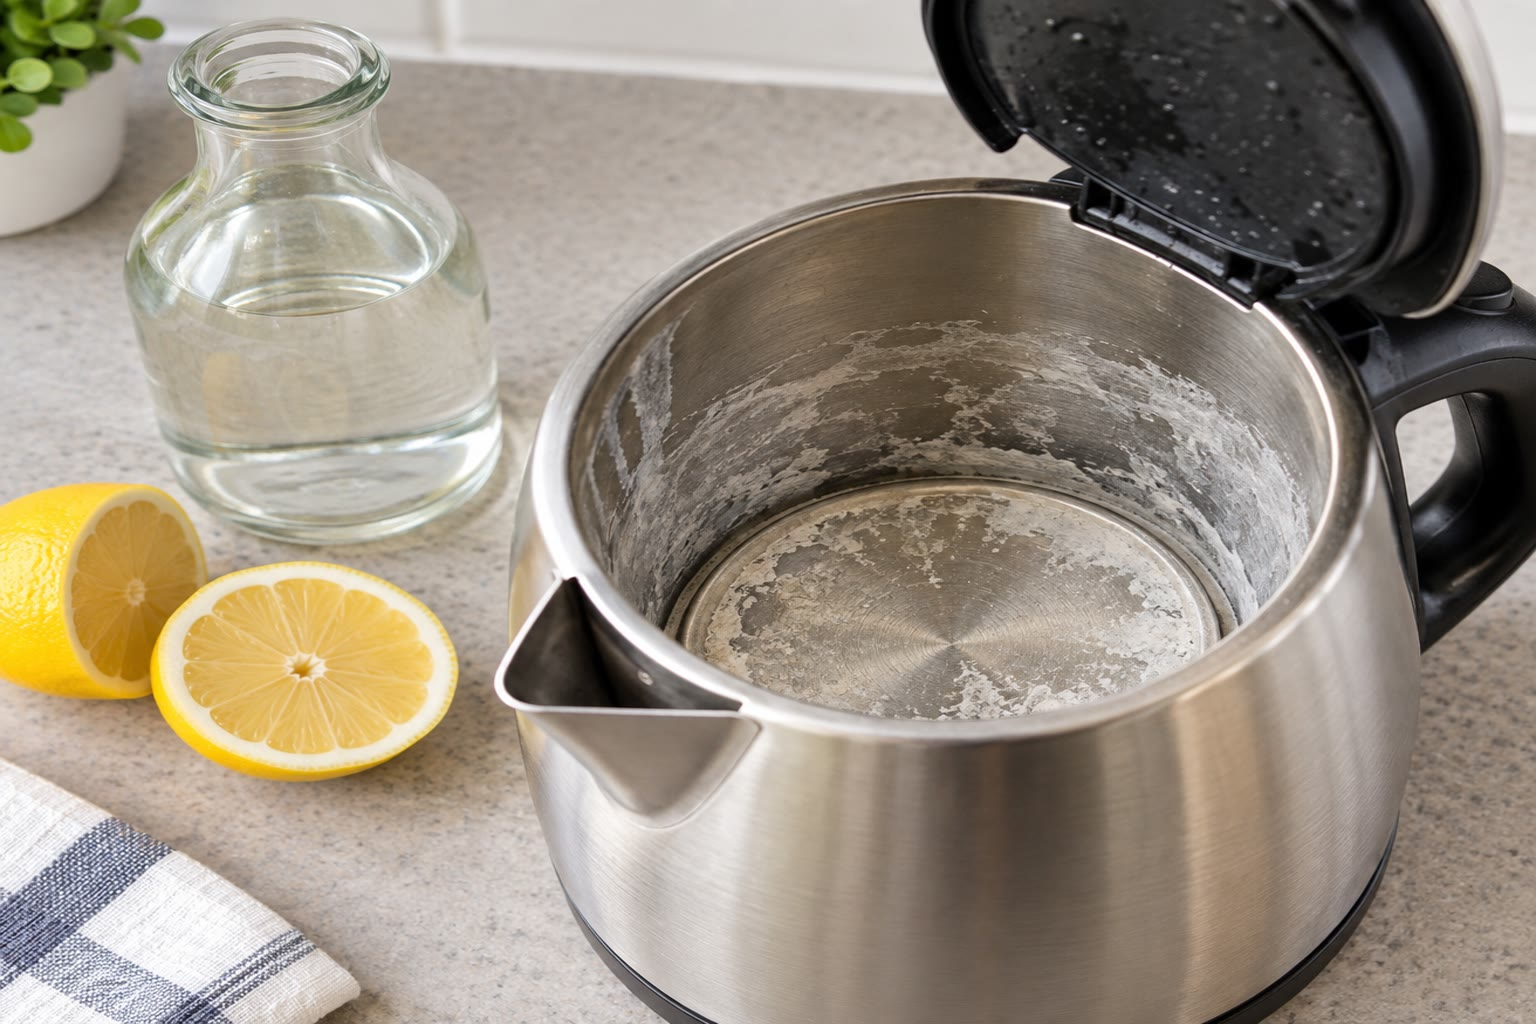
\includegraphics[width=0.5\linewidth]{images/book2/ai/b1-10-descaling.jpg}

{\small Calcário, carbonato de cálcio, em uma chaleira. Os \omterm{def:b1:predominant-reaction:strong-acid}{ácidos fracos}
do vinagre e do suco de limão reagem com o íon carbonato e o dissolvem.}
\end{omfigure}

\section{Pares de Brønsted e o pH}

\begin{definition}[Ácido e base de Brønsted, par]\label{def:b1:predominant-reaction:bronsted}
Um \emph{ácido de Brønsted}\index{acido de Bronsted@ácido de Brønsted} é uma espécie capaz de
ceder um próton \ce{H+}; uma \emph{base de Brønsted}\index{base de Bronsted@base de Brønsted} é
uma espécie capaz de aceitar um. Um ácido HA e a base A em que ele se
transforma ao perder um próton formam um \emph{par
ácido--base}\index{par acido--base@par ácido--base} HA/A, relacionados pela semiequação
formal $\mathrm{HA} \rightleftharpoons
\mathrm{A} + \ce{H+}$. Na água, o próton nunca fica livre: ele é
transportado por uma molécula de água na forma de \ce{H3O+}.
\end{definition}

\begin{definition}[Anfólito]\label{def:b1:predominant-reaction:ampholyte}
Um \emph{anfólito}\index{anfolito@anfólito} (uma espécie anfótera) é a base de um
par e o ácido de outro: a água (\ce{H3O+}/\ce{H2O} e \ce{H2O}/\ce{OH-}),
o íon hidrogenocarbonato (\ce{CO2,H2O}/\ce{HCO3-} e
\ce{HCO3-}/\ce{CO3^{2-}}), o íon di-hidrogenofosfato.
\end{definition}

\begin{definition}[Autoprotólise, produto iônico, pH]\label{def:b1:predominant-reaction:autoprotolysis}
A água sofre \emph{autoprotólise}\index{autoprotolise@autoprotólise},
\ce{2H2O <=> H3O+ + OH-}, de constante $K_e = [\ce{H3O+}][\ce{OH-}]$, o
\emph{produto iônico da água}\index{produto ionico da agua@produto iônico da água}; a
\qty{25}{\celsius}, $K_e = 10^{-14.00}$, logo $\mathrm{p}K_e = 14.00$. O
pH de uma solução é $\mathrm{pH} = -\log a(\ce{H3O+}) \approx -\log[\ce{H3O+}]$.
Uma solução é neutra quando $[\ce{H3O+}] = [\ce{OH-}]$, isto é, em
$\mathrm{pH} = \mathrm{p}K_e/2 = 7.00$ a \qty{25}{\celsius}.
% ledger: dfg:H2O_l, dfg:OH-_ao (pKe computed in figdata/bachelor-1/aqueous-constants.py)
\end{definition}

\section{Força: \texorpdfstring{$K_a$}{Ka}, \texorpdfstring{p$K_a$}{pKa} e o efeito nivelador}

\begin{definition}[Constante de acidez]\label{def:b1:predominant-reaction:acidity-constant}
A \emph{constante de acidez}\index{constante de acidez} de um par HA/A é
a constante da reação do ácido com a água,
\[
  \mathrm{HA} + \ce{H2O} \rightleftharpoons \mathrm{A} + \ce{H3O+}, \qquad
  K_a = \frac{[\mathrm{A}][\ce{H3O+}]}{[\mathrm{HA}]}, \qquad
  \mathrm{p}K_a = -\log K_a .
\]
Quanto maior $K_a$ (quanto menor o $\mathrm{p}K_a$), mais forte é o
ácido e mais fraca é sua base conjugada.
\end{definition}

\begin{definition}[Ácidos e bases fortes e fracos]\label{def:b1:predominant-reaction:strong-acid}
Um ácido é \emph{forte}\index{acido forte@ácido forte} em água se sua reação com a
água é total: não resta nenhuma molécula HA (ácidos clorídrico, nítrico,
perclórico, a primeira acidez do ácido sulfúrico); caso contrário, ele é
\emph{fraco}\index{acido fraco@ácido fraco}. Uma base é \emph{forte}\index{base forte}
se sua reação com a água é total, dando \ce{OH-} (hidróxidos, o íon
óxido, os alcóxidos), e \emph{fraca}\index{base fraca} caso contrário.
\end{definition}

\begin{definition}[Efeito nivelador]\label{def:b1:predominant-reaction:levelling}
Na água, todo ácido mais forte que \ce{H3O+} reage totalmente, dando
\ce{H3O+}, e toda base mais forte que \ce{OH-} reage totalmente, dando
\ce{OH-}: suas forças não podem ser distinguidas. É o \emph{efeito
nivelador}\index{efeito nivelador} do solvente. Os ácidos e as bases
fracos em água têm $0 < \mathrm{p}K_a < 14$, sendo a escala limitada
pelos pares da própria água
($\mathrm{p}K_a(\ce{H3O+}/\ce{H2O}) = 0$ e
$\mathrm{p}K_a(\ce{H2O}/\ce{OH-}) = 14$).
\end{definition}

\begin{center}
\small
\begin{tabular}{lll@{\hspace{2.5em}}lll}
\hline
par & p$K_a$ & & par & p$K_a$ & \\
\hline
\ce{HSO4-}/\ce{SO4^{2-}} & 1.99 & & \ce{CO2,H2O}/\ce{HCO3-} & 6.37 & \\
\ce{H3PO4}/\ce{H2PO4-} & 2.15 & & \ce{H2PO4-}/\ce{HPO4^{2-}} & 7.21 & \\
\ce{HF}/\ce{F-} & 3.16 & & \ce{HClO}/\ce{ClO-} & 7.55 & \\
\ce{HCOOH}/\ce{HCOO-} & 3.74 & & \ce{NH4+}/\ce{NH3} & 9.25 & \\
\ce{CH3COOH}/\ce{CH3COO-} & 4.76 & & \ce{C6H5OH}/\ce{C6H5O-} & 9.99 & \\
\ce{C6H5NH3+}/\ce{C6H5NH2} & 4.60 & & \ce{HCO3-}/\ce{CO3^{2-}} & 10.33 & \\
\ce{C6H5COOH}/\ce{C6H5COO-} & 4.21 & & \ce{CH3NH3+}/\ce{CH3NH2} & 10.66 & \\
\hline
\end{tabular}
\end{center}
% ledger: pka:methanoic, pka:ethanoic, pka:anilinium, pka:benzoic,
% pka:phenol, pka:methylammonium (IUPAC dataset); dfg:HSO4-_ao,
% dfg:SO42-_ao, dfg:H3PO4_ao, dfg:H2PO4-_ao, dfg:HPO42-_ao, dfg:HF_ao,
% dfg:F-_ao, dfg:CO2_ao, dfg:HCO3-_ao, dfg:CO32-_ao, dfg:HClO_ao,
% dfg:ClO-_ao, dfg:NH4+_ao, dfg:NH3_ao (pKa computed from NBS-82)

\section{Diagramas de predominância e de distribuição}

\begin{definition}[Diagramas de predominância e de distribuição]\label{def:b1:predominant-reaction:predominance}
Para um par HA/A, $\mathrm{pH} = \mathrm{p}K_a + \log([\mathrm{A}]/[\mathrm{HA}])$:
o ácido predomina ($[\mathrm{HA}] > [\mathrm{A}]$) para
$\mathrm{pH} < \mathrm{p}K_a$, a base para $\mathrm{pH} > \mathrm{p}K_a$.
O \emph{diagrama de predominância}\index{diagrama de predominancia@diagrama de predominância} é o eixo
de pH dividido, em cada $\mathrm{p}K_a$, nos domínios em que cada forma
predomina. O \emph{diagrama de distribuição}\index{diagrama de distribuicao@diagrama de distribuição}
dá a fração de cada forma, $[\text{forma}]/C$, em função do pH.
\end{definition}

\begin{proposition}[A relação de Henderson e as frações]\label{prop:b1:predominant-reaction:henderson}
Para um par HA/A de concentração total $C = [\mathrm{HA}] + [\mathrm{A}]$,
\[
  \mathrm{pH} = \mathrm{p}K_a + \log\frac{[\mathrm{A}]}{[\mathrm{HA}]}, \qquad
  \frac{[\mathrm{HA}]}{C} = \frac{1}{1 + 10^{\mathrm{pH} - \mathrm{p}K_a}}, \qquad
  \frac{[\mathrm{A}]}{C} = \frac{1}{1 + 10^{\mathrm{p}K_a - \mathrm{pH}}} .
\]
A uma unidade de pH do $\mathrm{p}K_a$, a forma minoritária fica abaixo
de 10\,\% do total; a duas unidades, abaixo de 1\,\%.
\end{proposition}

\begin{proof}
Tome o logaritmo de $K_a = [\mathrm{A}][\ce{H3O+}]/[\mathrm{HA}]$. Então
$[\mathrm{A}]/[\mathrm{HA}] = 10^{\mathrm{pH}-\mathrm{p}K_a}$, e dividir
$[\mathrm{HA}]$ por $[\mathrm{HA}] + [\mathrm{A}]$ dá as frações. Em
$\mathrm{pH} = \mathrm{p}K_a + 1$, $[\mathrm{HA}]/C = 1/11 < 10\,\%$; em
$+2$, $1/101$.
\end{proof}

\begin{omfigure}
\begin{tikzpicture}
\begin{axis}[name=e,
  width=0.48\linewidth, height=5.2cm, xmin=0, xmax=14, ymin=0, ymax=1.05,
  axis x line=bottom, axis y line=left, xlabel={pH}, ylabel={fração},
  xtick={0,2,4,6,8,10,12,14},
  tick label style={font=\small}, label style={font=\small}]
\addplot[omDef, thick] table[x=pH, y=HA] {figdata/out/bachelor-1-distribution-diagrams-ethanoic.dat};
\addplot[omThm, thick] table[x=pH, y=A] {figdata/out/bachelor-1-distribution-diagrams-ethanoic.dat};
\draw[dotted] (axis cs:4.76,0) -- (axis cs:4.76,0.5);
\node[omDef, font=\footnotesize, anchor=west] at (axis cs:0.3,0.3) {\ce{CH3COOH}};
\node[omThm, font=\footnotesize, anchor=east] at (axis cs:13.7,0.3) {\ce{CH3COO-}};
\node[font=\small, anchor=north west] at (axis cs:4.8,0.48) {4.76};
\end{axis}
\begin{axis}[at={(e.east)}, anchor=west, xshift=1.1cm,
  width=0.48\linewidth, height=5.2cm, xmin=0, xmax=14, ymin=0, ymax=1.05,
  axis x line=bottom, axis y line=left, xlabel={pH}, ylabel={fração},
  xtick={0,2,4,6,8,10,12,14},
  legend style={font=\scriptsize, draw=none, at={(0.5,1.04)}, anchor=south, legend columns=4},
  tick label style={font=\small}, label style={font=\small}]
\addplot[omDef, thick] table[x=pH, y=H3A] {figdata/out/bachelor-1-distribution-diagrams-phosphoric.dat};
\addplot[omMeth, thick] table[x=pH, y=H2A] {figdata/out/bachelor-1-distribution-diagrams-phosphoric.dat};
\addplot[omProp, thick] table[x=pH, y=HA] {figdata/out/bachelor-1-distribution-diagrams-phosphoric.dat};
\addplot[omThm, thick] table[x=pH, y=A] {figdata/out/bachelor-1-distribution-diagrams-phosphoric.dat};
\legend{\ce{H3PO4}, \ce{H2PO4-}, \ce{HPO4^{2-}}, \ce{PO4^{3-}}}

\end{axis}
\end{tikzpicture}

\begin{tikzpicture}[font=\small, >={Stealth}]
  \draw[->, thick] (0,0) -- (14.2*0.85,0) node[right] {pH};
  \foreach \x/\l in {2.15/2.15, 7.21/7.21, 12.34/12.34}
    \draw (\x*0.85,0.15) -- (\x*0.85,-0.15) node[below] {\l};
  \node[above] at (1.07*0.85,0.1) {\ce{H3PO4}};
  \node[above] at (4.68*0.85,0.1) {\ce{H2PO4-}};
  \node[above] at (9.78*0.85,0.1) {\ce{HPO4^{2-}}};
  \node[above] at (13.3*0.85,0.1) {\ce{PO4^{3-}}};
\end{tikzpicture}

{\small \omterm{def:b1:predominant-reaction:predominance}{Diagramas de distribuição} do ácido etanoico (à esquerda) e do
ácido fosfórico (à direita), e o \omterm{def:b1:predominant-reaction:predominance}{diagrama de predominância} do ácido
fosfórico. Cada cruzamento de duas curvas vizinhas fica em um
$\mathrm{p}K_a$; os \omterm{def:b1:predominant-reaction:ampholyte}{anfólitos} \ce{H2PO4-} e \ce{HPO4^{2-}} são quase a
única forma no meio de seus domínios.}
\end{omfigure}

\section{O método da reação predominante}

\begin{proposition}[Constante de uma reação ácido--base]\label{prop:b1:predominant-reaction:k-of-reaction}
A reação do ácido $\mathrm{HA}_1$ de um par com a base $\mathrm{A}_2$ de
outro,
$\mathrm{HA}_1 + \mathrm{A}_2 \rightleftharpoons \mathrm{A}_1 + \mathrm{HA}_2$,
tem a constante
\[
  K = \frac{K_{a1}}{K_{a2}} = 10^{\,\mathrm{p}K_{a2} - \mathrm{p}K_{a1}} .
\]
Ela é favorável ($K > 1$) quando o ácido é mais forte que o ácido que se
forma ($\mathrm{p}K_{a1} < \mathrm{p}K_{a2}$), e \omterm{def:b1:extent-q-and-k:quantitative}{quantitativa} (no sentido
do \cref{met:b1:extent-q-and-k:quantitative}) quando a diferença de
$\mathrm{p}K_a$ ultrapassa cerca de 4.
\end{proposition}

\begin{proof}
A reação é a soma de $\mathrm{HA}_1 + \ce{H2O} \rightleftharpoons
\mathrm{A}_1 + \ce{H3O+}$ ($K_{a1}$) e da inversa de $\mathrm{HA}_2 +
\ce{H2O} \rightleftharpoons \mathrm{A}_2 + \ce{H3O+}$ ($1/K_{a2}$); a
\cref{prop:b1:extent-q-and-k:combine-k} dá $K = K_{a1}/K_{a2}$.
\end{proof}

\begin{definition}[Reação predominante, solução equivalente]\label{def:b1:predominant-reaction:predominant-reaction}
Em uma solução que contém vários ácidos e bases, a \emph{reação
predominante}\index{reacao predominante@reação predominante} é a reação de maior constante
entre o ácido mais forte e a base mais forte presentes. Quando ela é
\omterm{def:b1:extent-q-and-k:quantitative}{quantitativa}, é tratada como total, e a solução é substituída pela
\emph{solução equivalente}\index{solucao equivalente@solução equivalente}: a solução obtida
depois que essa reação se completa, que tem o mesmo pH que a solução
real.
\end{definition}

\begin{method}[O método da reação predominante]\label{met:b1:predominant-reaction:method}
Para encontrar o pH e a composição de uma solução:
\begin{enumerate}
  \item liste as espécies introduzidas (e a água) e coloque seus pares em
        uma escala de $\mathrm{p}K_a$, os ácidos de um lado, as bases do
        outro;
  \item encontre o ácido mais forte e a base mais forte presentes;
  \item se a constante de sua reação for grande ($K > 10^4$, ou
        $\Delta\mathrm{p}K_a > 4$), trate a reação como total e escreva
        a \omterm{def:b1:predominant-reaction:predominant-reaction}{solução equivalente}; volte à etapa 2;
  \item quando a \omterm{def:b1:predominant-reaction:predominant-reaction}{reação predominante} tiver constante pequena, ela fixa o
        pH: monte sua tabela de avanço e resolva $Q = K$, em geral com a
        hipótese de que seu avanço é pequeno;
  \item verifique as hipóteses: as espécies minoritárias são de fato
        minoritárias, e as outras reações (inclusive a \omterm{def:b1:predominant-reaction:autoprotolysis}{autoprotólise} da
        água) são desprezíveis.
\end{enumerate}
\end{method}

\begin{omfigure}
\begin{tikzpicture}[font=\small, >={Stealth}]
  \draw[->, thick] (0,-0.3) -- (0,7.6) node[above] {p$K_a$};
  \foreach \y/\a/\b in {0/\ce{H3O+}/\ce{H2O}, 1.58/\ce{HF}/\ce{F-}, 2.38/\ce{CH3COOH}/\ce{CH3COO-},
      3.62/\ce{H2PO4-}/\ce{HPO4^{2-}}, 4.62/\ce{NH4+}/\ce{NH3}, 7/\ce{H2O}/\ce{OH-}} {
    \draw (-0.12,\y) -- (0.12,\y);
    \node[anchor=east] at (-0.2,\y) {\a};
    \node[anchor=west] at (0.2,\y) {\b};
  }
  \foreach \y/\l in {0/0, 1.58/3.16, 2.38/4.76, 3.62/7.21, 4.62/9.25, 7/14} \node[black!60, anchor=west] at (3.0,\y) {\l};
  \draw[->, omThm, thick] (-1.6,2.55) -- (1.2,4.45);
  \node[omThm, anchor=west, align=left] at (4.2,3.5) {um ácido reage com qualquer\\base situada acima dele: $K > 1$};
  \node[anchor=south] at (-1.4,7.35) {ácidos};
  \node[anchor=south] at (1.2,7.35) {bases};
\end{tikzpicture}

{\small Uma escala de $\mathrm{p}K_a$ (desenhada com o p$K_a$ crescendo
para cima; valores à direita). Um ácido reage favoravelmente com
qualquer base situada acima dele na escala: aqui, o ácido etanoico com a
amônia, $K = 10^{9.25 - 4.76} = 10^{4.49}$.}
\end{omfigure}

\begin{proposition}[pH de soluções simples]\label{prop:b1:predominant-reaction:ph-formulas}
À concentração $C$ (em \unit{mol/L}), com $\mathrm{p}C = -\log C$:
\begin{itemize}
  \item \omterm{def:b1:predominant-reaction:strong-acid}{ácido forte}: $\mathrm{pH} = \mathrm{p}C$, válido para
        $\mathrm{pH} < 6.5$;
  \item \omterm{def:b1:predominant-reaction:strong-acid}{ácido fraco}, pouco dissociado: $\mathrm{pH} = \frac12(\mathrm{p}K_a
        + \mathrm{p}C)$, válido se $\mathrm{pH} < \mathrm{p}K_a - 1$;
  \item \omterm{def:b1:predominant-reaction:strong-acid}{base fraca}, pouco protonada: $\mathrm{pH} = \frac12(\mathrm{p}K_e +
        \mathrm{p}K_a - \mathrm{p}C)$, válido se $\mathrm{pH} > \mathrm{p}K_a +
        1$;
  \item \omterm{def:b1:predominant-reaction:ampholyte}{anfólito} com $\mathrm{p}K_{a2} - \mathrm{p}K_{a1} > 4$:
        $\mathrm{pH} = \frac12(\mathrm{p}K_{a1} + \mathrm{p}K_{a2})$,
        qualquer que seja $C$ (se não for muito diluído).
\end{itemize}
\end{proposition}

\begin{proof}
\omterm{def:b1:predominant-reaction:strong-acid}{Ácido forte}: \ce{HA + H2O -> A- + H3O+} é total, $[\ce{H3O+}] = C$,
sendo a contribuição da própria água ($10^{-7}$) desprezível se $C > 10^{-6.5}$.
\omterm{def:b1:predominant-reaction:strong-acid}{Ácido fraco}: a \omterm{def:b1:predominant-reaction:predominant-reaction}{reação predominante} é $\mathrm{HA} + \ce{H2O}
\rightleftharpoons \mathrm{A} + \ce{H3O+}$, com avanço $x = [\ce{H3O+}]
= [\mathrm{A}]$; se $x \ll C$, $K_a = x^2/C$, $\mathrm{pH} = \frac12(\mathrm{p}K_a
+ \mathrm{p}C)$; a hipótese $[\mathrm{A}] < [\mathrm{HA}]/10$ equivale a
$\mathrm{pH} < \mathrm{p}K_a - 1$. \omterm{def:b1:predominant-reaction:strong-acid}{Base fraca}: o mesmo com $\mathrm{A} +
\ce{H2O} \rightleftharpoons \mathrm{HA} + \ce{OH-}$, de constante $K_e/K_a$.
\omterm{def:b1:predominant-reaction:ampholyte}{Anfólito} HA$^-$: a \omterm{def:b1:predominant-reaction:predominant-reaction}{reação predominante} é $2\,\mathrm{HA}^- \rightleftharpoons
\mathrm{H_2A} + \mathrm{A}^{2-}$, logo $[\mathrm{H_2A}] = [\mathrm{A}^{2-}]$;
multiplicar $K_{a1} = [\mathrm{HA}^-]h/[\mathrm{H_2A}]$ por $K_{a2} =
[\mathrm{A}^{2-}]h/[\mathrm{HA}^-]$ dá $h^2 = K_{a1}K_{a2}$.
\end{proof}

\begin{omfigure}
\begin{tikzpicture}
\begin{axis}[
  width=0.66\linewidth, height=5.6cm, xmin=0, xmax=8, ymin=0, ymax=8,
  axis x line=bottom, axis y line=left,
  xlabel={$\mathrm{p}C = -\log C$}, ylabel={pH},
  xtick={0,1,2,3,4,5,6,7,8}, ytick={0,1,2,3,4,5,6,7,8},
  tick label style={font=\small}, label style={font=\small},
  legend style={font=\small, draw=none, at={(0.02,0.98)}, anchor=north west}]
\addplot[omDef, very thick] table[x=pC, y=pH] {figdata/out/bachelor-1-weak-acid-ph.dat};
\addplot[omProp, dashed] table[x=pC, y=weak] {figdata/out/bachelor-1-weak-acid-ph.dat};
\addplot[black!50, dotted, thick] table[x=pC, y=strong] {figdata/out/bachelor-1-weak-acid-ph.dat};
\draw[black!30] (axis cs:0,7) -- (axis cs:8,7);
\legend{exato, $\frac12(\mathrm{p}K_a + \mathrm{p}C)$, $\mathrm{pH} = \mathrm{p}C$}
\end{axis}
\end{tikzpicture}

{\small pH de soluções de ácido etanoico em função de $\mathrm{p}C$,
calculado exatamente a partir do balanço de cargas. Concentrado, o ácido
é pouco dissociado e segue $\frac12(\mathrm{p}K_a + \mathrm{p}C)$;
diluído abaixo de cerca de $10^{-6}$ mol/L, ele está totalmente
dissociado e se comporta como um \omterm{def:b1:predominant-reaction:strong-acid}{ácido forte}; muito diluído, o pH tende
a 7.}
\end{omfigure}

\begin{example}[Ácido etanoico e amônia]\label{ex:b1:predominant-reaction:mixture}
Misture \qty{0.10}{mol} de ácido etanoico e \qty{0.10}{mol} de amônia em
\qty{1.0}{L}. O ácido mais forte é \ce{CH3COOH}, a base mais forte é
\ce{NH3}: \ce{CH3COOH + NH3 <=> CH3COO- + NH4+}, $K = 10^{9.25 - 4.76} =
10^{4.49}$, \omterm{def:b1:extent-q-and-k:quantitative}{quantitativa}. A \omterm{def:b1:predominant-reaction:predominant-reaction}{solução equivalente} contém
\qty{0.10}{mol/L} de \ce{CH3COO-} e de \ce{NH4+}. Sua \omterm{def:b1:predominant-reaction:predominant-reaction}{reação
predominante}, \ce{NH4+ + CH3COO- <=> NH3 + CH3COOH}, tem a pequena
constante $10^{-4.49}$ e mantém $[\ce{NH3}] = [\ce{CH3COOH}]$, donde,
como para um \omterm{def:b1:predominant-reaction:ampholyte}{anfólito}, $\mathrm{pH} = \frac12(4.76 + 9.25) = 7.01$.
\end{example}

\section{Poliácidos e tampões}

\begin{definition}[Poliácido]\label{def:b1:predominant-reaction:polyprotic}
Um \emph{poliácido}\index{poliacido@poliácido} pode ceder vários prótons
sucessivamente, cada etapa com sua própria constante: o ácido fosfórico
\ce{H3PO4} ($\mathrm{p}K_a$ = 2.15, 7.21, 12.34), o ácido carbônico
(\ce{CO2,H2O}; 6.37, 10.33), o ácido sulfúrico (primeira acidez forte,
segunda 1.99). Os $\mathrm{p}K_a$ sucessivos aumentam: retirar um próton
de uma espécie que já é negativa custa mais.
\end{definition}

\begin{example}[O ácido fosfórico a \texorpdfstring{\qty{0.10}{mol/L}}{0.10 mol/L}]\label{ex:b1:predominant-reaction:h3po4}
A \omterm{def:b1:predominant-reaction:predominant-reaction}{reação predominante} é a primeira acidez. Com $x = [\ce{H3O+}]$,
$x^2/(0.10 - x) = 10^{-2.15}$; aqui $x$ não é pequeno diante de $C$, de
modo que se resolve a equação do segundo grau $x^2 + K_{a1}x - K_{a1}C = 0$: $x =
\qty{0.0233}{mol/L}$, $\mathrm{pH} = 1.63$. A segunda acidez
($\mathrm{p}K_{a2} = 7.21$) não contribui em nada nesse pH.
\end{example}

\begin{definition}[Solução-tampão]\label{def:b1:predominant-reaction:buffer}
Uma \emph{solução-tampão}\index{solucao-tampao@solução-tampão} é uma solução cujo pH
varia pouco quando se adiciona uma pequena quantidade de ácido ou de
base, ou quando ela é diluída. O tampão usual é uma mistura de um \omterm{def:b1:predominant-reaction:strong-acid}{ácido
fraco} e de sua base conjugada em quantidades comparáveis; seu pH é
próximo do $\mathrm{p}K_a$ do par.
\end{definition}

\begin{proposition}[Por que um tampão resiste]\label{prop:b1:predominant-reaction:buffer}
Para um tampão de $n_a$ mol de ácido e $n_b$ mol de base, $\mathrm{pH} =
\mathrm{p}K_a + \log(n_b/n_a)$ não depende do volume. A adição de
$\delta$ mol de um \omterm{def:b1:predominant-reaction:strong-acid}{ácido forte} o faz variar de
\[
  \Delta\mathrm{pH} = \log\frac{n_b - \delta}{n_a + \delta} - \log\frac{n_b}{n_a}
  \approx -\frac{\delta}{\ln 10}\left(\frac{1}{n_a} + \frac{1}{n_b}\right),
\]
que é mínima para $n_a = n_b$, a quantidade total dada.
\end{proposition}

\begin{proof}
O \omterm{def:b1:predominant-reaction:strong-acid}{ácido forte} reage totalmente com a base: $n_b \to n_b - \delta$,
$n_a \to n_a + \delta$. A derivada de $f(\delta) = \log(n_b - \delta) -
\log(n_a + \delta)$ em 0 é $-\frac{1}{\ln10}\big(\frac{1}{n_b} +
\frac{1}{n_a}\big)$; para $n_a + n_b$ fixo, $\frac1{n_a} + \frac1{n_b}$ é
mínima quando $n_a = n_b$.
\end{proof}

\begin{definition}[Grau de dissociação]\label{def:b1:predominant-reaction:dissociation}
O \emph{grau de dissociação}\index{grau de dissociacao@grau de dissociação} de um \omterm{def:b1:predominant-reaction:strong-acid}{ácido fraco}
HA de concentração analítica $C$ é $\alpha = [\mathrm{A}]/C$, a fração do
ácido dissociada pela água; ele satisfaz a lei da diluição de Ostwald,
$\alpha^2C/(1 - \alpha) = K_a$, e tende a 1 quando $C \to 0$.
\end{definition}

\begin{inthelab}[Preparar um tampão]
Um tampão é preparado no laboratório pesando o ácido e seu sal (por
exemplo, o di-hidrogenofosfato de sódio e o hidrogenofosfato
dissódico), ou adicionando ao ácido um volume medido de solução de
hidróxido de sódio enquanto se lê um pHmetro, calibrado antes com dois
tampões padrão; a solução é então completada até o traço de aferição em
um balão volumétrico.
\end{inthelab}

\section{Exercícios}

\begin{exercise}[$\star$]\label{exo:b1:predominant-reaction:1}
Escreva a base conjugada de \ce{H2SO4}, \ce{HCO3-}, \ce{NH4+} e
\ce{H2O}, e o ácido conjugado de \ce{NH3}, \ce{HPO4^{2-}}, \ce{OH-} e
\ce{H2O}. Quais dessas espécies são \omterm{def:b1:predominant-reaction:ampholyte}{anfólitos}?
\end{exercise}

\begin{exercise}[$\star$]\label{exo:b1:predominant-reaction:2}
Usando a tabela de $\mathrm{p}K_a$, ordene por força o ácido fluorídrico,
o ácido etanoico, o íon amônio e o ácido hipocloroso, e dê o $K_a$ de
cada um.
\end{exercise}

\begin{exercise}[$\star$]\label{exo:b1:predominant-reaction:3}
Calcule o pH de uma solução de ácido clorídrico a \qty{0.010}{mol/L} e
de uma solução de hidróxido de sódio a \qty{0.010}{mol/L}, a
\qty{25}{\celsius}.
\end{exercise}

\begin{exercise}[$\star$]\label{exo:b1:predominant-reaction:4}
Desenhe o \omterm{def:b1:predominant-reaction:predominance}{diagrama de predominância} do par \ce{CH3COOH}/\ce{CH3COO-}.
Que forma predomina em um refrigerante de pH 3? E no sangue, de pH 7.4?
Que fração do ácido está na forma ácida em pH 3.76?
\end{exercise}

\begin{exercise}[$\star\star$]\label{exo:b1:predominant-reaction:5}
Calcule o pH de uma solução de amônia a \qty{0.10}{mol/L} e verifique a
hipótese feita.
\end{exercise}

\begin{exercise}[$\star\star$]\label{exo:b1:predominant-reaction:6}
Calcule o pH de uma solução de ácido etanoico a \qty{0.010}{mol/L} e o
\omterm{def:b1:predominant-reaction:dissociation}{grau de dissociação}; verifique a hipótese.
\end{exercise}

\begin{exercise}[$\star\star$]\label{exo:b1:predominant-reaction:7}
Escreva a \omterm{def:b1:predominant-reaction:predominant-reaction}{reação predominante}, sua constante e o pH de uma solução
obtida misturando, em \qty{1.0}{L}, \qty{0.10}{mol} de ácido fluorídrico
e \qty{0.050}{mol} de hidróxido de sódio.
\end{exercise}

\begin{exercise}[$\star\star$]\label{exo:b1:predominant-reaction:8}
Um tampão contém \qty{0.050}{mol} de ácido etanoico e \qty{0.050}{mol}
de etanoato de sódio em \qty{1.0}{L}. Calcule seu pH e, depois, o pH após
a adição de \qty{0.010}{mol} de ácido clorídrico. Compare com a mesma
adição a \qty{1.0}{L} de água pura.
\end{exercise}

\begin{exercise}[$\star\star$]\label{exo:b1:predominant-reaction:9}
Os ácidos clorídrico e nítrico têm a mesma força na água, mas não no
ácido etanoico puro como solvente. Explique e diga qual é o ácido mais
forte que pode existir na água.
\end{exercise}

\begin{exercise}[$\star\star\star$]\label{exo:b1:predominant-reaction:10}
Calcule o pH de uma solução de carbonato de sódio a \qty{0.10}{mol/L} e
verifique que a segunda basicidade pode ser desprezada.
\end{exercise}

\begin{exercise}[$\star\star\star$]\label{exo:b1:predominant-reaction:11}
Demonstre a lei da diluição de Ostwald e calcule o \omterm{def:b1:predominant-reaction:dissociation}{grau de dissociação}
do ácido etanoico em $C = \qty{1.0e-3}{mol/L}$. Por que a aproximação
$\alpha \ll 1$ falha aqui?
\end{exercise}

\begin{exercise}[$\star\star\star$]\label{exo:b1:predominant-reaction:12}
Uma solução contém \qty{0.010}{mol/L} de ácido clorídrico e
\qty{0.10}{mol/L} de ácido etanoico. Encontre seu pH e a concentração de
íons etanoato; explique por que o \omterm{def:b1:predominant-reaction:strong-acid}{ácido fraco} quase não se dissocia.
\end{exercise}

\section{Problema: Um tampão fosfato para o laboratório de cultura de células}

\begin{problem}[{Problema de fim de semana --- as três acidezes do ácido
fosfórico, o pH de seus três sais de sódio, as soluções equivalentes e o
volume de hidróxido de sódio que dá um tampão de pH 7.20}]
\label{pb:b1:predominant-reaction:1}
As células cultivadas em laboratório precisam de um meio com pH próximo
de 7.2. Dados a \qty{25}{\celsius}: $\mathrm{p}K_a$ do ácido fosfórico
2.15, 7.21 e
12.34; $\mathrm{p}K_e = 14.00$.

\medskip
\noindent\textbf{Parte I --- O ácido fosfórico.}
\begin{enumerate}
  \item Escreva os três pares e suas semiequações.
  \item Desenhe o \omterm{def:b1:predominant-reaction:predominance}{diagrama de predominância} do ácido fosfórico.
  \item Que espécie predomina em pH 1, 5, 9 e 13?
  \item Quais espécies são \omterm{def:b1:predominant-reaction:ampholyte}{anfólitos}?
  \item Por que cada $\mathrm{p}K_a$ é maior que o anterior?
\end{enumerate}

\medskip
\noindent\textbf{Parte II --- Três soluções a \qty{0.100}{mol/L}.}
\begin{enumerate}[resume]
  \item Para o ácido fosfórico, escreva a \omterm{def:b1:predominant-reaction:predominant-reaction}{reação predominante} e mostre que
        seu avanço não é desprezível diante de $C$.
  \item Calcule o pH da solução de ácido fosfórico.
  \item Para o di-hidrogenofosfato de sódio \ce{NaH2PO4}, escreva a \omterm{def:b1:predominant-reaction:predominant-reaction}{reação
        predominante} e sua constante.
  \item Calcule o pH dessa solução.
  \item Calcule o pH de uma solução de hidrogenofosfato dissódico
        \ce{Na2HPO4}.
  \item Qual das três soluções está mais próxima do pH desejado?
\end{enumerate}

\medskip
\noindent\textbf{Parte III --- Adição de hidróxido de sódio.}
Uma solução contém \qty{0.100}{mol} de \ce{H3PO4}; adicionam-se $n$ mol
de hidróxido de sódio, com volume total de \qty{1.00}{L}.
\begin{enumerate}[resume]
  \item Escreva a reação dos primeiros \qty{0.100}{mol} de hidróxido e sua
        constante. Ela é \omterm{def:b1:extent-q-and-k:quantitative}{quantitativa}?
  \item Descreva a \omterm{def:b1:predominant-reaction:predominant-reaction}{solução equivalente} para $n = \qty{0.100}{mol}$ e dê
        seu pH.
  \item Mesma pergunta para $n = \qty{0.150}{mol}$.
  \item Mesma pergunta para $n = \qty{0.200}{mol}$.
  \item Esboce o pH em função de $n$ de 0 a \qty{0.300}{mol}.
  \item Por que a solução da questão 14 é um bom tampão?
\end{enumerate}

\medskip
\noindent\textbf{Parte IV --- Preparar \qty{1.00}{L} de tampão de pH 7.20.}
Dispõe-se de hidróxido de sódio a \qty{1.00}{mol/L}.
\begin{enumerate}[resume]
  \item Que razão $[\ce{HPO4^{2-}}]/[\ce{H2PO4-}]$ dá pH 7.20?
  \item Expresse as quantidades de \ce{H2PO4-} e de \ce{HPO4^{2-}} em
        função da quantidade $x$ de hidróxido adicionada além dos
        primeiros \qty{0.100}{mol}.
  \item Calcule $x$.
  \item De quanto varia o pH se \qty{1.0e-3}{mol} de ácido clorídrico
        for adicionado a esse tampão? E a \qty{1.00}{L} de água pura?
  \item O pH variaria se o tampão fosse diluído dez vezes? Explique.
  \item Calcule o volume de solução de hidróxido de sódio a adicionar a
        \qty{0.100}{mol} de ácido fosfórico para obter \qty{1.00}{L} de
        tampão de pH 7.20.
\end{enumerate}
\end{problem}
